Em um aeroporto, os passageiros devem submeter suas bagagens a uma das cinco m�quinas de raio-X dispon�veis ao adentrarem a sala de embarque. Num dado instante, o tempo gasto por essas m�quinas para escanear a bagagem de cada passageiro e o n�mero de pessoas presentes em cada fila est�o apresentados em um painel, como mostrado na figura.
\begin{figure}[h]
\caption{Exemplo}
\centering
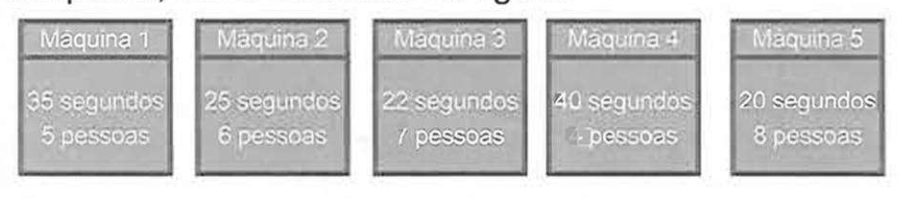
\includegraphics[width=8cm]{../figuras/q138-2018.png}
\label{Figura:1}
\end{figure}

Um passageiro, ao chegar � sala de embarque desse aeroporto no instante indicado, visando esperar o menor tempo poss�vel, dever� se dirigir � m�quina.

\begin{enumerate}
\item[a)]1
\item[b)]2
\item[c)]3
\item[d)]4
\item[e)]5
\end{enumerate}
